\setcounter{ex}{0}
\setcounter{vd}{0}
\section*{ÔN TẬP THPTQG 2026 - XÁC SUẤT CÓ ĐIỀU KIỆN}
\subsection{Ví dụ}
\Opensolutionfile{ans}[ans/DA-CD5-XAC-SUAT-CO-DIEU-KIEN-VD]
\begin{vd} % Bài 6.2
    Cho $P(A) = 0,2$; $P(B) = 0,51$; $P(B | A) = 0,8$. Tính $P(A | B)$.
    \choice
    { $\dfrac{8}{51}$ }
    {\True $\dfrac{16}{51}$ }
    { $\dfrac{4}{15}$ }
    { $\dfrac{16}{255}$ }
    \loigiai{
        Ta có $P(A \cap B) = P(A) \cdot P(B|A) = 0,2 \cdot 0,8 = 0,16$.
        Xác suất cần tìm: $P(A|B) = \dfrac{P(A \cap B)}{P(B)} = \dfrac{0,16}{0,51} = \dfrac{16}{51}$.
    }
    %\dotlineEX{1}
\end{vd}
\begin{vd} % Bài 6.1
    Một hộp kín đựng 20 tấm thẻ giống hệt nhau đánh số từ 1 đến 20. Một người rút ngẫu nhiên ra một tấm thẻ từ trong hộp. Người đó được thông báo rằng thẻ rút ra mang số chẵn. Tính xác suất để người đó rút được thẻ số 10.
    \choice
    { $\dfrac{1}{20}$ }
    { $\dfrac{1}{2}$ }
    {\True $\dfrac{1}{10}$ }
    { $\dfrac{1}{5}$ }
    \loigiai{
        Gọi $A$ là biến cố "Rút được thẻ số 10", $B$ là biến cố "Thẻ rút ra mang số chẵn".
        Ta có $B = \{2, 4, 6, 8, 10, 12, 14, 16, 18, 20\} \Rightarrow n(B) = 10$.
        Vì thẻ số 10 là số chẵn nên $A \cap B = A$. Xác suất cần tìm là $P(A|B) = \dfrac{n(A \cap B)}{n(B)} = \dfrac{1}{10}$.
    }
    %\dotlineEX{1}
\end{vd}
\begin{vd}[BGD-2025]%[2D6H2-4]
    Một phần mềm nhận dạng tin nhắn quảng cáo trên điện thoại bằng cách dựa theo từ khóa để đánh dấu một số tin nhắn được gửi đến. Qua một thời gian dài sử dụng, người ta thấy rằng trong số tất cả các tin nhắn gửi đến, có $15 \%$ số tin nhắn bị đánh dấu. Trong số các tin nhắn bị đánh dấu, có $10 \%$ số tin nhắn không phải là quảng cáo. Trong số các tin nhắn không bị đánh dấu, có $5 \%$ số tin nhắn là quảng cáo.
    Chọn ngẫu nhiên một tin nhắn được gửi đến điện thoại.
    \choiceTF
    {\True Xác suất để tin nhắn đó không bị đánh dấu bằng $0{,}85$}
    {\True Xác suất để tin nhắn đó không phải là quảng cáo, biết rằng nó không bị đánh dấu, bằng $0{,}95$}
    {Xác suất để tin nhắn đó không phải là quảng cáo bằng $0{,}85$}
    {\True Xác suất để tin nhắn đó không bị đánh dấu, biết rằng nó không phải là quảng cáo, lớn hơn $0{,}95$}
    \loigiai{
        Gọi $A$ là biến cố \lq\lq Tin nhắn bị đánh dấu\rq\rq ; $B$ là biến cố \lq\lq Tin nhắn là quảng cáo\rq\rq .\\
        Theo giả thiết, ta có sơ đồ hình cây sau đây
        \begin{center}
            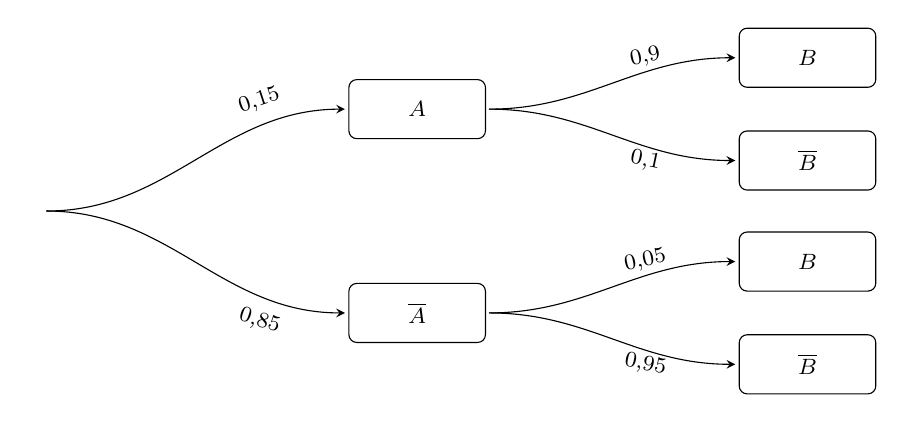
\begin{tikzpicture}[line join = round, line cap = round, >=stealth, font=\footnotesize, scale=1]
                \def\gocm{15}\def\gocn{7.5}\def\r{5}
                \tikzset{s/.style={outer sep=0.5 mm,draw=black,rectangle,minimum width=1.5cm,text width=1.5cm,align=center,rounded corners=1mm,minimum height=0.75cm}}
                
                \path(0,0)node(O){}++(\gocm:\r)node[s](A1){$A$}++(\gocn:\r)node[s](A2){$B$};
                \path(A1)++({-\gocn}:\r)node[s](a2){$\overline{B}$};
                \path(O)++(-\gocm:\r)node[s](B1){$\overline{A}$}++(\gocn:\r)node[s](B2){$B$};
                \path(B1)++({-\gocn}:\r)node[s](b2){$\overline{B}$};
                \foreach \x/\y in {O/A1,A1/A2,A1/a2,O/B1,B1/B2,B1/b2}{
                    \draw[->,out=0,in=180] (\x.east)to(\y.west);	}
                \path
                (O)--(A1.west)node[pos=0.75,above=2mm,sloped]{$0{,}15$} (A1.east)--(A2.west)node[pos=0.65,above,sloped]{$0{,}9$}
                (A1.east)--(a2.west)node[pos=0.65,below,sloped]{$0{,}1$}
                (O)--(B1.west)node[pos=0.75,below=2mm,sloped]{$0{,}85$}
                (B1.east)--(B2.west)node[pos=0.65,above,sloped]{$0{,}05$}
                (B1.east)--(b2.west)node[pos=0.65,below,sloped]{$0{,}95$}
                ;
            \end{tikzpicture}
        \end{center}
        \begin{itemchoice}
            \itemch  Xác suất để tin nhắn không bị đánh dấu là $\mathrm{P}\left(\overline{A}\right)=1-\mathrm{P}(A)=1-0{,}15=0{,}85$.
            \itemch  Xác suất để tin nhắn không phải là quảng cáo, biết rằng nó không bị đánh dấu là $$\mathrm{P}\left(\overline{B}\mid\overline{A}\right)=1-\mathrm{P}\left(B|\overline{A}\right)=1-0{,}05=0{,}95.$$
            \itemch  Xác suất để tin nhắn không phải là quảng cáo là
            \allowdisplaybreaks
            \begin{eqnarray*}
                \mathrm{P}\left(\overline{B}\right)&=&\mathrm{P}(A)\cdot \mathrm{P}\left(\overline{B}\mid A\right) + \mathrm{P}\left(\overline{A}\right)\cdot \mathrm{P}\left(\overline{B}\mid \overline{A}\right)\\
                &=& 0{,}15 \cdot 0{,}1 + 0{,}85 \cdot 0{,}95 = 0{,}8225.
            \end{eqnarray*}
            \itemch  Xác suất để tin nhắn không bị đánh dấu, biết rằng nó không phải là quảng cáo là
            $$\mathrm{P}\left(\overline{A}\mid \overline{B}\right)=\dfrac{\mathrm{P}\left(\overline{A}\right)\cdot \mathrm{P}\left(\overline{B}|\overline{A}\right)}{\mathrm{P}\left(\overline{B}\right)}=\dfrac{0{,}85 \cdot 0{,}95}{0{,}8225}\approx 0{,}98.$$
            Vậy $\mathrm{P}\left(\overline{A}\mid \overline{B}\right) > 0{,}95$.
        \end{itemchoice}
    }
    %\dotlineEX{4}
\end{vd}
\begin{vd} % Bài 6.18
    Để thử nghiệm tác dụng điều trị bệnh mất ngủ của hai loại thuốc X và thuốc Y, người ta tiến hành thử nghiệm trên 4000 người bệnh tình nguyện. Kết quả cho thấy: Thuốc X có 1600 người khỏi, 800 người không khỏi; Thuốc Y có 1200 người khỏi, 400 người không khỏi. Chọn ngẫu nhiên 1 người bệnh tham gia thử nghiệm.
    \choiceTF
    {\True Tổng số người dùng thuốc X là 2400 người}
    { Xác suất người đó khỏi bệnh nếu biết người đó uống thuốc X là $0,5$}
    {\True Tổng số người khỏi bệnh trong thử nghiệm là 2800 người}
    { Xác suất người đó uống thuốc Y, biết rằng người đó khỏi bệnh là $\dfrac{4}{7}$}
    \loigiai{
        Tổng số người dùng thuốc X = $1600+800=2400$. (Ý a đúng)
        Ý b: $P(\text{Khỏi} | X) = \dfrac{1600}{2400} = \dfrac{2}{3}$ (Sai).
        Ý c: Tổng số người khỏi bệnh = $1600+1200=2800$ (Đúng).
        Ý d: $P(Y | \text{Khỏi}) = \dfrac{1200}{2800} = \dfrac{3}{7}$ (Sai).
    }
\end{vd}
\begin{vd} % Bài 6.6
    Trong một túi có một số chiếc kẹo cùng loại, chỉ khác màu, trong đó có 6 cái kẹo màu cam, còn lại là kẹo màu vàng. Hà lấy ngẫu nhiên một cái kẹo từ trong túi, không trả lại. Sau đó Hà lại lấy ngẫu nhiên thêm một cái kẹo khác. Biết rằng xác suất Hà lấy được cả hai cái kẹo màu cam là $\dfrac{1}{3}$. Hỏi ban đầu trong túi có bao nhiêu cái kẹo?\shortans{10}
    \loigiai{
        Gọi số kẹo ban đầu trong túi là $n$ ($n > 6$).
        Xác suất lấy lần 1 được kẹo cam là $\dfrac{6}{n}$.
        Sau khi lấy 1 kẹo cam, trong túi còn $n-1$ kẹo, trong đó có 5 kẹo cam. Xác suất lấy lần 2 kẹo cam là $\dfrac{5}{n-1}$.
        Xác suất lấy 2 kẹo cam: $\dfrac{6}{n} \cdot \dfrac{5}{n-1} = \dfrac{1}{3} \Leftrightarrow n(n-1) = 90 \Leftrightarrow n^2 - n - 90 = 0 \Rightarrow n = 10$.
        \textbf{Đáp án:} 10
    }
\end{vd}
\begin{vd}[Minh hoạ BGD-2025]%[Câu 6]
    Có hai chiếc hộp, hộp I có $6$ quả bóng màu đỏ và $4$ quả bóng màu vàng, hộp II có $7$ quả bóng màu đỏ và $3$ quả bóng màu vàng, các quả bóng có cùng kích thước và khối lượng. Lấy ngẫu nhiên một quả bóng từ hộp I bỏ vào hộp II. Sau đó, lấy ra ngẫu nhiên một quả bóng từ hộp II. Tính xác suất để quả bóng được lấy ra từ hộp II là quả bóng được chuyển từ hộp I sang, biết rằng quả bóng đó có màu đỏ (làm tròn kết quả đến hàng phần trăm).
    \shortans{0,08}
    \loigiai{
        Gọi $T$ là biến cố "Quả bóng chuyển từ hộp I sang hộp II là màu đỏ".
        Xác suất $P(T) = \dfrac{6}{10} = 0.6$.
        Xác suất quả bóng chuyển sang màu vàng là $P(\overline{T}) = \dfrac{4}{10} = 0.4$.
        Gọi $D$ là biến cố "Quả bóng lấy ra từ hộp II là màu đỏ".
        Ta có xác suất để lấy được bóng đỏ từ hộp II là:
        $P(D) = P(D|T)P(T) + P(D|\overline{T})P(\overline{T})$
        Nếu $T$ xảy ra (chuyển bóng đỏ), hộp II có 8 đỏ, 3 vàng $\Rightarrow P(D|T) = \dfrac{8}{11}$.
        Nếu $\overline{T}$ xảy ra (chuyển bóng vàng), hộp II có 7 đỏ, 4 vàng $\Rightarrow P(D|\overline{T}) = \dfrac{7}{11}$.
        Suy ra $P(D) = \dfrac{8}{11} \times \dfrac{6}{10} + \dfrac{7}{11} \times \dfrac{4}{10} = \dfrac{76}{110}$.
        Gọi $S$ là biến cố "Quả bóng lấy ra từ hộp II chính là quả bóng được chuyển từ hộp I sang".
        Ta cần tính xác suất điều kiện $P(S|D) = \dfrac{P(S \cap D)}{P(D)}$.
        Biến cố $S \cap D$ nghĩa là "Quả bóng chuyển sang là màu đỏ VÀ quả bóng lấy ra chính là quả bóng đó".
        Xác suất chuyển bóng đỏ là $\dfrac{6}{10}$. Khi đã chuyển sang, hộp II có 11 quả bóng, xác suất để bốc trúng đúng quả vừa chuyển là $\dfrac{1}{11}$.
        Do đó, $P(S \cap D) = \dfrac{6}{10} \times \dfrac{1}{11} = \dfrac{6}{110}$.
        Vậy xác suất cần tìm là:
        $P(S|D) = \dfrac{\dfrac{6}{110}}{\dfrac{76}{110}} = \dfrac{6}{76} = \dfrac{3}{38} \approx 0.08$.
        \hfill \textbf{Đáp số:} $0.08$.
    }
%    %\dotlineEX{2}
\end{vd}
\begin{vd} % Bài 6.7
    Trong quân sự, một máy bay chiến đấu có thể xuất hiện ở vị trí X với xác suất $0,55$. Nếu máy bay không xuất hiện ở vị trí X thì nó xuất hiện ở vị trí Y. Nếu máy bay xuất hiện tại X thì bắn 2 quả tên lửa, tại Y thì bắn 1 quả. Biết xác suất bắn trúng của mỗi tên lửa là $0,8$ và hoạt động độc lập. Máy bay bị bắn hạ nếu trúng ít nhất 1 quả tên lửa. Tính xác suất bắn hạ máy bay đối phương (kết quả làm tròn đến hàng phần trăm).\shortans{0,89}
    \loigiai{
        Xác suất máy bay ở X là $0,55$, ở Y là $0,45$.
        Nếu ở X, bắn 2 quả. Xác suất bắn hạ (trúng ít nhất 1 quả) là $1 - (1-0,8)^2 = 0,96$.
        Nếu ở Y, bắn 1 quả. Xác suất bắn hạ là $0,8$.
        Xác suất bắn hạ máy bay: $P = 0,55 \cdot 0,96 + 0,45 \cdot 0,8 = 0,528 + 0,36 = 0,888$.
        \textbf{Đáp án:} 0,888
    }
\end{vd}
\begin{vd} % Bài 6.20
    Chuồng I có 5 con gà mái, 2 con gà trống. Chuồng II có 3 con gà mái, 5 con gà trống. Bác Mai bắt một con gà theo cách sau: Tung một con xúc xắc. Nếu số chấm chia hết cho 3 thì chọn chuồng I, nếu không thì chọn chuồng II. Sau đó bắt ngẫu nhiên một con từ chuồng đã chọn. Tính xác suất bắt được gà mái (làm tròn đến hàng phần trăm). \shortans{0,49}
   \loigiai{
       Mặt xúc xắc chia hết cho 3 là $\{3, 6\}$. Xác suất chọn chuồng I là $\dfrac{2}{6} = \dfrac{1}{3}$. Xác suất chọn chuồng II là $\dfrac{2}{3}$.
       - Chuồng I: Xác suất bắt được gà mái là $\dfrac{5}{7}$.
       - Chuồng II: Xác suất bắt được gà mái là $\dfrac{3}{8}$.
       Xác suất bắt được gà mái là: $P = \dfrac{1}{3} \cdot \dfrac{5}{7} + \dfrac{2}{3} \cdot \dfrac{3}{8} = \dfrac{5}{21} + \dfrac{6}{24} = \dfrac{41}{84}$.
    %    \textbf{Đáp án:} 41/84
   }
\end{vd}
\Closesolutionfile{ans}
\Opensolutionfile{ans}[ans/DA-CD5-XAC-SUAT-CO-DIEU-KIEN-BTRL]
\subsection{Bài tập}
\begin{ex}%[134706] [MĐ1]
    Cho hai biến cố $A$ và $B$. Công thức nào sau đây là công thức đúng tính xác suất của biến cố $A$ với điều kiện $B$?
    \choice
    {\True $P(A|B) = \dfrac{P(AB)}{P(B)}$}
    {$P(A|B) = \dfrac{P(A \cup B)}{P(B)}$}
    {$P(A|B) = \dfrac{P(AB)}{P(A)}$}
    {$P(A|B) = \dfrac{P(A \cup B)}{P(A)}$}
%    \loigiai{
%        Theo định nghĩa xác suất có điều kiện, ta có $P(A|B) = \dfrac{P(AB)}{P(B)}$ (với $P(B) > 0$).
%    }
\end{ex}
\begin{ex}%[134710] [MĐ1]
    Cho hai biến cố $A$ và $B$ là hai biến cố độc lập. Khẳng định nào dưới đây là đúng?
    \choice
    {$P(A) = P(B)$}
    {$P(A) \cdot P(B) = P(A|B)$}
    {\True $P(A|B) = P(A)$}
    {$P(B|A) = P(A)$}
%    \loigiai{
%        Vì $A$ và $B$ là hai biến cố độc lập nên sự xảy ra của $B$ không ảnh hưởng đến xác suất xảy ra của $A$. Do đó $P(A|B) = P(A)$.
%    }
\end{ex}
\begin{ex}%[360681] [MĐ1]
    Cho hai biến cố xung khắc $A, B$ với $P(A) = 0,2; P(B) = 0,4$. Khi đó, $P(A|B)$ bằng
    \choice
    {$0,5$}
    {$0,2$}
    {$0,4$}
    {\True $0$}
%    \loigiai{
%        Vì $A, B$ xung khắc nên $P(AB) = 0$. Khi đó $P(A|B) = \dfrac{P(AB)}{P(B)} = \dfrac{0}{0,4} = 0$.
%    }
\end{ex}
\begin{ex}%[360664] [MĐ1]
    Cho hai biến cố độc lập $A, B$ với $P(A) = 0,8; P(B) = 0,25$. Khi đó, $P(A|B)$ bằng
    \choice
    {$0,2$}
    {\True $0,8$}
    {$0,25$}
    {$0,75$}
%    \loigiai{
%        Vì $A, B$ độc lập nên $P(A|B) = P(A) = 0,8$.
%    }
\end{ex}
\begin{ex}%[134718] [MĐ1]
    Nếu $P(A) = 0,3; P(B) = 0,4; P(AB) = 0,1$ thì $P(A|B)$ bằng
    \choice
    {$0,4$}
    {$0,3$}
    {\True $0,25$}
    {$0,7$}
    \loigiai{
        Ta có $P(A|B) = \dfrac{P(AB)}{P(B)} = \dfrac{0,1}{0,4} = 0,25$.
    }
\end{ex}
\begin{ex}%[143806] [MĐ2]
    Cho $P(A) = \dfrac{2}{7}$; $P(B|A) = \dfrac{1}{4}$; $P(B|\overline{A}) = \dfrac{1}{5}$. Giá trị $P(B)$ là
    \choice
    {$\dfrac{1}{7}$}
    {\True $\dfrac{3}{14}$}
    {$\dfrac{1}{14}$}
    {$\dfrac{2}{7}$}
    \loigiai{
        Ta có $P(\overline{A}) = 1 - P(A) = 1 - \dfrac{2}{7} = \dfrac{5}{7}$.\\
        Theo công thức xác suất toàn phần:
        $$P(B) = P(A)P(B|A) + P(\overline{A})P(B|\overline{A}) = \dfrac{2}{7} \cdot \dfrac{1}{4} + \dfrac{5}{7} \cdot \dfrac{1}{5} = \dfrac{2}{28} + \dfrac{5}{35} = \dfrac{1}{14} + \dfrac{1}{7} = \dfrac{3}{14}.$$
    }
    %\dotlineEX{1}
\end{ex}
\begin{ex}%[135717] [MĐ2]
    Thống kê $2000$ sinh viên một khóa của trường đại học theo giới tính và ngành học thu được các số liệu sau:
    \begin{center}
        \begin{tabular}{|l|c|c|}
            \hline
            & Nam & Nữ \\
            \hline
            Học tài chính ngân hàng & $400$ & $500$ \\
            \hline
            Học quản trị kinh doanh & $800$ & $300$ \\
            \hline
        \end{tabular}
    \end{center}
    Lấy ngẫu nhiên một sinh viên khóa đó. Nếu đã chọn được một sinh viên nam hãy tính xác suất để người đó học tài chính ngân hàng bằng bao nhiêu?
    \choice
    {$\dfrac{1}{5}$}
    {$\dfrac{1}{2}$}
    {\True $\dfrac{1}{3}$}
    {$\dfrac{2}{5}$}
    \loigiai{
        Tổng số sinh viên nam là $400 + 800 = 1200$.\\
        Số sinh viên nam học tài chính ngân hàng là $400$.\\
        Xác suất cần tìm: $P = \dfrac{400}{1200} = \dfrac{1}{3}$.
    }
\end{ex}
\begin{ex}%[135722] [MĐ2]
    Khảo sát $100$ người trong đó có $49$ nam và $51$ nữ về việc có nuôi thú cưng không thì được bảng sau:
    \begin{center}
        \begin{tabular}{|l|c|c|c|}
            \hline
            & Có thú cưng & Không có thú cưng & Tổng \\
            \hline
            Nam & $41$ & $8$ & $49$ \\
            \hline
            Nữ & $45$ & $6$ & $51$ \\
            \hline
            Tổng & $86$ & $14$ & $100$ \\
            \hline
        \end{tabular}
    \end{center}
    Chọn ngẫu nhiên một người trong số người được khảo sát. Biết người đó là nam, tính xác suất của biến cố người được chọn nuôi thú cưng?
    \choice
    {$\dfrac{41}{86}$}
    {\True $\dfrac{41}{49}$}
    {$\dfrac{41}{100}$}
    {$\dfrac{1763}{2450}$}
%    \loigiai{
%        Theo bảng số liệu, tổng số nam là $49$ người. Số nam có nuôi thú cưng là $41$ người.\\
%        Xác suất cần tìm là $P = \dfrac{41}{49}$.
%    }
\end{ex}
\begin{ex}%[135724] [MĐ2]
    Một hộp chứa 8 bi trắng, 2 bi đỏ. Lần lượt bốc từng bi theo phương thức không hoàn lại. Giả sử lần đầu tiên bốc được bi trắng. Xác suất lần thứ 2 bốc được bi đỏ là
    \choice
    {$\dfrac{1}{9}$}
    {\True $\dfrac{2}{9}$}
    {$\dfrac{3}{9}$}
    {$\dfrac{4}{9}$}
%    \loigiai{
%        Sau khi bốc lần đầu được bi trắng và không hoàn lại, trong hộp còn $7$ bi trắng và $2$ bi đỏ. Tổng cộng còn $9$ viên.\\
%        Xác suất để lần thứ 2 bốc được bi đỏ là $P = \dfrac{2}{9}$.
%    }
%\dotlineEX{1}
\end{ex}
\begin{ex}%[360669] [MĐ2]
    Một lô sản phẩm có 20 sản phẩm, trong đó có 5 sản phẩm chất lượng thấp. Lấy liên tiếp 2 sản phẩm trong lô sản phẩm trên, trong đó sản phẩm lấy ra ở lần thứ nhất không được bỏ lại vào lô sản phẩm. Tính xác suất để cả hai sản phẩm được lấy ra đều có chất lượng thấp.
    \choice
    {\True $\dfrac{1}{19}$}
    {$\dfrac{1}{20}$}
    {$\dfrac{5}{76}$}
    {$\dfrac{4}{19}$}
    \loigiai{
        Xác suất lần 1 lấy được sản phẩm thấp là $\dfrac{5}{20}$.\\
        Xác suất lần 2 lấy được sản phẩm thấp (khi đã lấy 1 sản phẩm thấp ra) là $\dfrac{4}{19}$.\\
        Xác suất cả 2 lần đều thấp là $P = \dfrac{5}{20} \cdot \dfrac{4}{19} = \dfrac{1}{19}$.
    }
\end{ex}
\begin{ex}%[143807] [MĐ2]
    Một học sinh đi học muộn với xác suất là $0,3$. Nếu người đó đi học muộn thì xác suất để người đó ăn sáng là $0,2$. Nếu người đó không đi học muộn thì xác suất để người đó ăn sáng là $0,6$. Ta có sơ đồ hình cây như hình bên. Xác suất của biến cố người đó ăn sáng là
    \begin{center}
        \begin{tikzpicture}
            \def\gocm{20}
            \def\gocn{10}
            \def\r{5}
            \tikzset{s/.style={outer sep=0.5 mm,draw=magenta,rectangle,minimum width=2.75cm,rounded corners=1mm}}
            \path(0,0)node(O){}++(\gocm:\r)node[s](A1){đi học muộn}++(\gocn:\r)node[s](A2){ăn sáng};
            \path(A1)++({-\gocn}:\r)node[s](a2){không ăn sáng};
            \path(O)++(-\gocm:\r)node[s](B1){không đi học muộn}++(\gocn:\r)node[s](B2){ăn sáng};
            \path(B1)++({-\gocn}:\r)node[s](b2){Không ăn sáng};
            \foreach \x/\y in {
                O/A1,A1/A2,
                O/B1,B1/B2,
                A1/a2,
                B1/b2}
            \draw[-stealth](\x.east)--(\y.west);
            \path(O)--(A1.west)node[pos=0.5,above,sloped]{$\mbox{0{,}3}$}(O)--(B1.west)node[pos=0.5,below]{$\mbox{0,7}$}(B1.east)--(B2.west)node[pos=0.5,above]{$\mbox{0,6}$}(A1.east)--(A2.west)node[pos=0.5,above]{$\mbox{0,2}$}
            (A1.east)--(a2.west)node[pos=0.5,below,sloped]{$\mbox{0{,}8}$}
            (B1.east)--(b2.west)node[pos=0.5,below,sloped]{$\mbox{0{,}4}$};
            %    %%Node dòng trên
            %    \path(A2)++(0,1)node{\textbf{Chủ nhật}}++(180:4)node{\textbf{Thứ bảy}};
        \end{tikzpicture}
    \end{center}
    \choice
    {\True $0,48$}
    {$0,8$}
    {$0,52$}
    {$0,9$}
    \loigiai{
        Gọi $M$ là biến cố "Học sinh đi học muộn", $\overline{M}$ là biến cố "Không đi học muộn".\\
        Gọi $A$ là biến cố "Học sinh ăn sáng".\\
        Theo công thức xác suất toàn phần:
        $$P(A) = P(M)P(A|M) + P(\overline{M})P(A|\overline{M}) = 0,3 \cdot 0,2 + 0,7 \cdot 0,6 = 0,06 + 0,42 = 0,48.$$
    }
\end{ex}
\begin{ex}%[143809] [MĐ2]
    Một cậu bé có một hộp bi gồm 6 viên bi đỏ và 4 viên bi trắng. Một hôm cậu thấy mất 1 viên bi mà không biết viên bi đó màu gì. Tính xác suất để khi lấy ngẫu nhiên ra một viên bi trong số còn lại từ hộp thì ta được bi đỏ.
    \choice
    {$0,5$}
    {$0,4$}
    {$0,7$}
    {\True $0,6$}
    \loigiai{
        Ban đầu hộp có 10 viên. Xác suất viên bi bị mất là đỏ: $P(M_D) = \dfrac{6}{10} = 0,6$. Xác suất bị mất là trắng: $P(M_T) = \dfrac{4}{10} = 0,4$.\\
        Gọi $A$ là biến cố "Lấy được viên bi đỏ từ 9 viên còn lại".
        \begin{itemize}
            \item Nếu mất bi đỏ: Hộp còn 5 đỏ, 4 trắng. Suy ra $P(A|M_D) = \dfrac{5}{9}$.
            \item Nếu mất bi trắng: Hộp còn 6 đỏ, 3 trắng. Suy ra $P(A|M_T) = \dfrac{6}{9}$.
        \end{itemize}
        Áp dụng công thức xác suất toàn phần:
        $$P(A) = P(M_D)P(A|M_D) + P(M_T)P(A|M_T) = 0,6 \cdot \dfrac{5}{9} + 0,4 \cdot \dfrac{6}{9} = \dfrac{3}{9} + \dfrac{2,4}{9} = \dfrac{5,4}{9} = 0,6.$$
    }
\end{ex}
\begin{ex}%[143810] [MĐ2]
    Hai nhà máy cùng sản xuất 1 loại linh kiện điện tử. Năng suất nhà máy hai gấp 3 lần năng suất nhà máy một. Tỷ lệ hỏng của nhà máy một và hai lần lượt là $0,1\%$ và $0,2\%$. Giả sử linh kiện bán ở Trung tâm chỉ do hai nhà máy này sản xuất. Mua 1 linh kiện ở Trung tâm. Tính xác suất để linh kiện ấy hỏng.
    \choice
    {\True $0,175\%$}
    {$0,125\%$}
    {$0,225\%$}
    {$0,233\%$}
    \loigiai{
        Vì năng suất nhà máy hai gấp 3 lần nhà máy một nên tỷ lệ linh kiện của nhà máy một là $\dfrac{1}{4} = 0,25$ và nhà máy hai là $\dfrac{3}{4} = 0,75$.\\
        Gọi $H$ là biến cố "Linh kiện bị hỏng". Ta có $P(H|NM_1) = 0,001$ và $P(H|NM_2) = 0,002$.\\
        Áp dụng công thức xác suất toàn phần:
        $$P(H) = 0,25 \cdot 0,001 + 0,75 \cdot 0,002 = 0,00025 + 0,00150 = 0,00175 = 0,175\%.$$
    }
\end{ex}
\begin{ex}%[143818] [MĐ2]
    Một xét nghiệm Covid-19 cho kết quả dương tính với $90\%$ các trường hợp thực sự nhiễm virus và cho kết quả âm tính với $80\%$ các trường hợp thực sự không nhiễm virus. Biết rằng tỉ lệ người nhiễm Covid-19 trong một cộng đồng nào đó là $1\%$. Một người trong cộng đồng đó có kết quả xét nghiệm dương tính. Xác suất để người đó thực sự bị nhiễm virus là
    \choice
    {\True $\dfrac{1}{23}$}
    {$\dfrac{8}{207}$}
    {$\dfrac{8}{23}$}
    {$\dfrac{11}{23}$}
    \loigiai{
        Gọi $N$ là biến cố "Người đó thực sự nhiễm virus", suy ra $P(N) = 0,01$ và $P(\overline{N}) = 0,99$.\\
        Gọi $D$ là biến cố "Kết quả xét nghiệm dương tính".\\
        Theo đề bài, $P(D|N) = 0,9$ và $P(\overline{D}|\overline{N}) = 0,8 \Rightarrow P(D|\overline{N}) = 1 - 0,8 = 0,2$.\\
        Xác suất để một người có kết quả dương tính là:
        $$P(D) = P(N)P(D|N) + P(\overline{N})P(D|\overline{N}) = 0,01 \cdot 0,9 + 0,99 \cdot 0,2 = 0,009 + 0,198 = 0,207.$$
        Xác suất người đó thực sự nhiễm bệnh khi có kết quả dương tính:
        $$P(N|D) = \dfrac{P(N \cap D)}{P(D)} = \dfrac{0,009}{0,207} = \dfrac{9}{207} = \dfrac{1}{23}.$$
    }
\end{ex}
\begin{ex}%[145260] [MĐ2]
    Kết quả khảo sát tại một xã cho thấy có $20\%$ cư dân hút thuốc lá. Tỉ lệ cư dân thường xuyên gặp các vấn đề sức khoẻ về đường hô hấp trong số những người hút thuốc lá và không hút thuốc lá lần lượt là $70\%$ và $15\%$. Nếu ta gặp một cư dân của xã thường xuyên gặp các vấn đề sức khoẻ về đường hô hấp thì xác suất người đó có hút thuốc lá là khoảng bao nhiêu phần trăm?
    \choice
    {$46\%$}
    {$58\%$}
    {$26\%$}
    {\True $54\%$}
    \loigiai{
        Gọi $H$ là biến cố "Người đó hút thuốc lá", $P(H) = 0,2 \Rightarrow P(\overline{H}) = 0,8$.\\
        Gọi $B$ là biến cố "Người đó gặp vấn đề đường hô hấp".\\
        Ta có $P(B|H) = 0,7$ và $P(B|\overline{H}) = 0,15$.\\
        Xác suất một người gặp vấn đề hô hấp:
        $$P(B) = P(H)P(B|H) + P(\overline{H})P(B|\overline{H}) = 0,2 \cdot 0,7 + 0,8 \cdot 0,15 = 0,14 + 0,12 = 0,26.$$
        Xác suất người đó hút thuốc khi biết người đó mắc bệnh:
        $$P(H|B) = \dfrac{P(H \cap B)}{P(B)} = \dfrac{0,14}{0,26} = \dfrac{7}{13} \approx 0,538 \approx 54\%.$$
    }
\end{ex}
\begin{ex}%[143819] [MĐ2]
    Tỷ lệ sản phẩm tốt của máy thứ nhất là $99\%$, của máy thứ hai là $98\%$. Một lô sản phẩm gồm $40\%$ sản phẩm của máy thứ nhất và $60\%$ sản phẩm của máy thứ hai. Người ta lấy ngẫu nhiên ra một sản phẩm để kiểm tra thấy là sản phẩm tốt. Tìm xác suất để sản phẩm đó do máy thứ nhất sản xuất.
    \choice
    {$\dfrac{123}{125}$}
    {$\dfrac{2}{125}$}
    {$\dfrac{49}{82}$}
    {\True $\dfrac{33}{82}$}
   \loigiai{
       Gọi $M_1, M_2$ lần lượt là biến cố sản phẩm do máy 1 và máy 2 sản xuất. $P(M_1) = 0,4$; $P(M_2) = 0,6$.\\
       Gọi $T$ là biến cố "Sản phẩm tốt". $P(T|M_1) = 0,99$; $P(T|M_2) = 0,98$.\\
       Xác suất lấy được sản phẩm tốt:
       $$P(T) = P(M_1)P(T|M_1) + P(M_2)P(T|M_2) = 0,4 \cdot 0,99 + 0,6 \cdot 0,98 = 0,396 + 0,588 = 0,984.$$
       Xác suất để sản phẩm tốt đó do máy 1 sản xuất:
       $$P(M_1|T) = \dfrac{P(M_1 \cap T)}{P(T)} = \dfrac{0,396}{0,984} = \dfrac{396}{984} = \dfrac{33}{82}.$$
   }
%\dotlineEX{2}
\end{ex}
\begin{ex}%[143820] [MĐ2]
    Tỷ lệ người nghiện thuốc là ở một vùng là $30\%$. Biết rằng tỷ lệ người bị viêm họng trong số những người nghiện thuốc là $60\%$, còn tỷ lệ người bị viêm họng trong số những người không nghiện là $40\%$. Lấy ngẫu nhiên một người thấy người ấy không bị viêm họng. Tính xác suất người đó nghiện thuốc lá.
    \choice
    {$\dfrac{14}{23}$}
    {\True $\dfrac{2}{9}$}
    {$\dfrac{7}{9}$}
    {$\dfrac{9}{23}$}
    \loigiai{
        Gọi $N$ là biến cố "Nghiện thuốc", $P(N) = 0,3 \Rightarrow P(\overline{N}) = 0,7$.\\
        Gọi $V$ là biến cố "Bị viêm họng". Theo đề: $P(V|N) = 0,6 \Rightarrow P(\overline{V}|N) = 0,4$ (không bị viêm họng).\\
        Và $P(V|\overline{N}) = 0,4 \Rightarrow P(\overline{V}|\overline{N}) = 0,6$.\\
        Xác suất chọn được người không bị viêm họng là:
        $$P(\overline{V}) = 0,3 \cdot 0,4 + 0,7 \cdot 0,6 = 0,12 + 0,42 = 0,54.$$
        Xác suất người đó nghiện thuốc biết rằng không bị viêm họng là:
        $$P(N|\overline{V}) = \dfrac{P(N \cap \overline{V})}{P(\overline{V})} = \dfrac{0,12}{0,54} = \dfrac{12}{54} = \dfrac{2}{9}.$$
    }
\end{ex}
\begin{ex}%[145262] [MĐ2]
    Một bệnh viện đang xét nghiệm cho một số bệnh nhân để xác định liệu họ có nhiễm virus X hay không. Xác suất để một bệnh nhân bị nhiễm virus X là $0,05$. Khi xét nghiệm, nếu một bệnh nhân bị nhiễm thì xác suất để kết quả xét nghiệm dương tính là $0,95$. Nếu một bệnh nhân không bị nhiễm thì xác suất để kết quả xét nghiệm âm tính là $0,98$. Một bệnh nhân được chọn ngẫu nhiên và có kết quả xét nghiệm dương tính. Xác suất để bệnh nhân đó thực sự bị nhiễm virus X là
    \choice
    {$\dfrac{133}{2000}$}
    {$\dfrac{19}{400}$}
    {\True $\dfrac{5}{7}$}
    {$\dfrac{2}{7}$}
    \loigiai{
        Gọi $N$ là biến cố "Nhiễm virus", $P(N) = 0,05 \Rightarrow P(\overline{N}) = 0,95$.\\
        Gọi $D$ là biến cố "Xét nghiệm dương tính".\\
        Ta có $P(D|N) = 0,95$ và $P(\overline{D}|\overline{N}) = 0,98 \Rightarrow P(D|\overline{N}) = 0,02$.\\
        Xác suất để có kết quả dương tính:
        $$P(D) = P(N)P(D|N) + P(\overline{N})P(D|\overline{N}) = 0,05 \cdot 0,95 + 0,95 \cdot 0,02 = 0,0475 + 0,0190 = 0,0665.$$
        Xác suất thực sự nhiễm bệnh khi kết quả dương tính:
        $$P(N|D) = \dfrac{P(N \cap D)}{P(D)} = \dfrac{0,0475}{0,0665} = \dfrac{475}{665} = \dfrac{5}{7}.$$
    }
\end{ex}
\begin{ex}%[145263] [MĐ2]
    Ở một địa phương X, xác suất để một người lớn trên 40 tuổi mắc bệnh ung thư là $0,05$. Xác suất bác sĩ chẩn đoán đúng một người mắc bệnh ung thư là $0,78$ và chẩn đoán sai (không bị ung thư nhưng được chẩn đoán mắc bệnh) là $0,06$. Xác suất để một người thật sự mắc bệnh ung thư khi nhận được kết quả chẩn đoán bị ung thư bằng
    \choice
    {\True $0,40625$}
    {$0,096$}
    {$0,904$}
    {$0,59375$}
    \loigiai{
        Gọi $U$ là biến cố "Mắc bệnh ung thư", $P(U) = 0,05 \Rightarrow P(\overline{U}) = 0,95$.\\
        Gọi $D$ là biến cố "Chẩn đoán mắc bệnh". Ta có $P(D|U) = 0,78$ và $P(D|\overline{U}) = 0,06$.\\
        Xác suất một người được chẩn đoán mắc bệnh là:
        $$P(D) = P(U)P(D|U) + P(\overline{U})P(D|\overline{U}) = 0,05 \cdot 0,78 + 0,95 \cdot 0,06 = 0,039 + 0,057 = 0,096.$$
        Xác suất thật sự mắc bệnh khi được chẩn đoán mắc bệnh:
        $$P(U|D) = \dfrac{P(U \cap D)}{P(D)} = \dfrac{0,039}{0,096} = \dfrac{39}{96} = \dfrac{13}{32} = 0,40625.$$
    }
\end{ex}
\begin{ex}%[143821] [MĐ2]
    Có hai đội thi đấu môn Bắn súng. Đội I có 6 vận động viên, đội II có 8 vận động viên. Xác suất đạt huy chương vàng của mỗi vận động viên đội I và đội II tương ứng là $0,65$ và $0,55$. Chọn ngẫu nhiên một vận động viên trong hai đội. Giả sử vận động viên được chọn đạt huy chương vàng. Tính xác suất để vận động viên này thuộc đội I.
    \choice
    {$\dfrac{39}{140}$}
    {\True $\dfrac{39}{83}$}
    {$\dfrac{43}{83}$}
    {$\dfrac{37}{140}$}
    \loigiai{
        Tổng số VĐV là $14$. Xác suất chọn được VĐV đội I là $P(I) = \dfrac{6}{14} = \dfrac{3}{7}$, đội II là $P(II) = \dfrac{8}{14} = \dfrac{4}{7}$.\\
        Gọi $V$ là biến cố "Vận động viên đạt huy chương vàng". $P(V|I) = 0,65$ và $P(V|II) = 0,55$.\\
        Xác suất chọn được VĐV đạt huy chương vàng:
        $$P(V) = \dfrac{3}{7} \cdot 0,65 + \dfrac{4}{7} \cdot 0,55 = \dfrac{1,95 + 2,2}{7} = \dfrac{4,15}{7}.$$
        Xác suất VĐV đó thuộc đội I là:
        $$P(I|V) = \dfrac{P(I \cap V)}{P(V)} = \dfrac{\dfrac{1,95}{7}}{\dfrac{4,15}{7}} = \dfrac{1,95}{4,15} = \dfrac{195}{415} = \dfrac{39}{83}.$$
    }
\end{ex}
\begin{ex}%[145269] [MĐ2]
    Trong một trường học, tỉ lệ học sinh nữ là $52\%$. Tỉ lệ học sinh nữ và tỉ lệ học sinh nam tham gia câu lạc bộ nghệ thuật lần lượt là $18\%$ và $15\%$. Gặp ngẫu nhiên 1 học sinh của trường. Biết rằng học sinh có tham gia câu lạc bộ nghệ thuật. Tính xác suất học sinh đó là nam.
    \choice
    {$\dfrac{17}{23}$}
    {$\dfrac{13}{23}$}
    {$\dfrac{15}{23}$}
    {\True $\dfrac{10}{23}$}
   \loigiai{
       Gọi $N\tilde{u}$ là biến cố "Học sinh nữ", $P(N\tilde{u}) = 0,52 \Rightarrow P(Nam) = 0,48$.\\
       Gọi $A$ là biến cố "Tham gia câu lạc bộ nghệ thuật". $P(A|N\tilde{u}) = 0,18$ và $P(A|Nam) = 0,15$.\\
       Xác suất học sinh tham gia câu lạc bộ:
       $$P(A) = 0,52 \cdot 0,18 + 0,48 \cdot 0,15 = 0,0936 + 0,0720 = 0,1656.$$
       Xác suất học sinh đó là nam biết rằng có tham gia CLB:
       $$P(Nam|A) = \dfrac{P(Nam \cap A)}{P(A)} = \dfrac{0,0720}{0,1656} = \dfrac{7200}{16560} = \dfrac{10}{23}.$$
   }
\end{ex}
\begin{ex}%[143822] [MĐ2]
    Túi I chứa 4 quả bóng trắng và 6 quả bóng đen, túi II khác chứa 4 quả bóng trắng và 3 quả bóng đen. Lấy ngẫu nhiên một quả bóng từ một trong các túi và thấy nó có màu đen. Xác suất để nó được rút ra từ Túi I bằng
    \choice
    {\True $\dfrac{7}{12}$}
    {$\dfrac{5}{12}$}
    {$\dfrac{3}{7}$}
    {$\dfrac{4}{7}$}
    \loigiai{
        Xác suất chọn mỗi túi là như nhau: $P(I) = P(II) = 0,5$.\\
        Gọi $Đ$ là biến cố "Rút được quả bóng đen". Ta có $P(Đ|I) = \dfrac{6}{10} = 0,6$; $P(Đ|II) = \dfrac{3}{7}$.\\
        Xác suất rút được bóng đen chung:
        $$P(Đ) = 0,5 \cdot 0,6 + 0,5 \cdot \dfrac{3}{7} = 0,3 + \dfrac{1,5}{7} = \dfrac{2,1 + 1,5}{7} = \dfrac{3,6}{7}.$$
        Xác suất quả bóng đen đó từ túi I:
        $$P(I|Đ) = \dfrac{P(I \cap Đ)}{P(Đ)} = \dfrac{0,3}{\dfrac{3,6}{7}} = \dfrac{2,1}{3,6} = \dfrac{21}{36} = \dfrac{7}{12}.$$
    }
\end{ex}
\begin{ex}%[144409] [MĐ2]
    Một người đàn ông được biết là cứ mỗi ba lần thì người đó sẽ nói sự thật 2 lần. Anh ta tung một con xúc xắc và báo cáo rằng kết quả mặt hiển thị là số 4 hay không là số 4. Tính xác suất để số thu được thực sự là số 4 khi anh ta báo cáo nó là số 4.
    \choice
    {$\dfrac{5}{6}$}
    {$\dfrac{1}{6}$}
    {$\dfrac{5}{7}$}
    {\True $\dfrac{2}{7}$}
    \loigiai{
        Xác suất người này nói sự thật là $P(T) = \dfrac{2}{3}$, xác suất nói dối là $P(D) = \dfrac{1}{3}$.\\
        Thực tế gieo xúc xắc: Xác suất ra số 4 là $P(S_4) = \dfrac{1}{6}$, không ra số 4 là $P(\overline{S_4}) = \dfrac{5}{6}$.\\
        Anh ta "báo cáo là số 4" (gọi là biến cố $B$) trong 2 trường hợp:
        \begin{itemize}
            \item Thực sự ra số 4 và anh ta nói thật: $P(S_4 \cap T) = \dfrac{1}{6} \cdot \dfrac{2}{3} = \dfrac{2}{18}$.
            \item Thực sự không ra số 4 và anh ta nói dối (biến thành báo số 4): $P(\overline{S_4} \cap D) = \dfrac{5}{6} \cdot \dfrac{1}{3} = \dfrac{5}{18}$.
        \end{itemize}
        Xác suất anh ta báo cáo là số 4: $P(B) = \dfrac{2}{18} + \dfrac{5}{18} = \dfrac{7}{18}$.\\
        Xác suất số thực sự là 4 khi báo cáo là 4:
        $$P(S_4|B) = \dfrac{\dfrac{2}{18}}{\dfrac{7}{18}} = \dfrac{2}{7}.$$
    }
\end{ex}
\begin{ex}%[144829] [MĐ2]
    Một nhà máy sản xuất bóng đèn có tỷ lệ bóng đèn đạt tiêu chuẩn là $80\%$. Trước khi xuất ra thị trường, mỗi bóng đèn đều được qua kiểm tra chất lượng. Vì sự kiểm tra không thể tuyệt đối hoàn hảo nên một bóng đèn tốt có xác suất $0,9$ được công nhận là tốt và một bóng đèn hỏng có xác suất $0,95$ bị loại bỏ. Tỷ lệ bóng đèn đạt tiêu chuẩn sau khi qua khâu kiểm tra chất lượng là bao nhiêu phần trăm. Làm tròn kết quả đến hàng phần chục.
    \choice
    {$96,8\%$}
    {$99,1\%$}
    {\True $98,6\%$}
    {$97,6\%$}
    \loigiai{
        Gọi $T$ là biến cố "Bóng đèn thực sự đạt tiêu chuẩn (tốt)", $P(T) = 0,8 \Rightarrow P(\overline{T}) = 0,2$ (hỏng).\\
        Gọi $C$ là biến cố "Bóng đèn được công nhận là tốt qua khâu kiểm tra".\\
        Theo đề bài: $P(C|T) = 0,9$. Bóng đèn hỏng bị loại với xác suất $0,95 \Rightarrow$ được công nhận tốt với xác suất $P(C|\overline{T}) = 1 - 0,95 = 0,05$.\\
        Tỷ lệ bóng đèn được công nhận là tốt (được tung ra thị trường):
        $$P(C) = P(T)P(C|T) + P(\overline{T})P(C|\overline{T}) = 0,8 \cdot 0,9 + 0,2 \cdot 0,05 = 0,72 + 0,01 = 0,73.$$
        Tỷ lệ bóng thực sự đạt tiêu chuẩn trong số những bóng đã được công nhận tốt (xuất ra thị trường):
        $$P(T|C) = \dfrac{P(T \cap C)}{P(C)} = \dfrac{0,72}{0,73} \approx 0,9863 \approx 98,6\%.$$
    }
    %\dotlineEX{1}
\end{ex}
\begin{ex}%[135802] [MĐ2]
    Bạn An có một túi kẹo, trong đó có 8 viên bi đen và 6 viên bi trắng. An lấy ngẫu nhiên 1 viên bi trong túi để cho Việt, rồi lại lấy ngẫu nhiên tiếp 1 viên bi nữa trong túi và cũng đưa cho Việt. Các mệnh đề sau đúng hay sai?
    \choiceTF
    {\True Xác suất để Việt nhận được 2 viên bi trắng là $\dfrac{15}{91}$}
    { Xác suất để Việt nhận được 2 viên bi đen là $\dfrac{2}{7}$}
    {\True Xác suất để Việt nhận được viên bi đen ở lần thứ nhất và viên bi trắng ở lần thứ hai là $\dfrac{24}{91}$}
    { Xác suất để Việt nhận được viên bi trắng ở lần thứ nhất và viên bi đen ở lần thứ hai là $\dfrac{12}{49}$}
    \loigiai{
        Tổng số bi trong túi ban đầu là $8 + 6 = 14$ viên.\\
        a) Lấy 2 viên bi trắng không hoàn lại: $P = \dfrac{6}{14} \cdot \dfrac{5}{13} = \dfrac{15}{91}$. (Đúng)\\
        b) Lấy 2 viên bi đen không hoàn lại: $P = \dfrac{8}{14} \cdot \dfrac{7}{13} = \dfrac{4}{13}$. Mệnh đề cho $\dfrac{2}{7}$, là sai.\\
        c) Đen lần 1, trắng lần 2: $P = \dfrac{8}{14} \cdot \dfrac{6}{13} = \dfrac{24}{91}$. (Đúng)\\
        d) Trắng lần 1, đen lần 2: $P = \dfrac{6}{14} \cdot \dfrac{8}{13} = \dfrac{24}{91}$. Mệnh đề cho $\dfrac{12}{49}$, là sai.
    }
    %\dotlineEX{2}
\end{ex}
\begin{ex}%[135806] [MĐ2]
    Ở một sân bay, người ta sử dụng một loại máy soi tự động phát hiện hàng cấm trong hành lí kí gửi. Máy phát chuông cảnh báo với 95\% các kiện hành lí có chứa hàng cấm và 2\% các kiện hành lí không chứa hàng cấm. Tỉ lệ các kiện hành lí có chứa hàng cấm là 1\%. Chọn ngẫu nhiên một kiện hành lí để soi bằng máy trên. Các mệnh đề sau đúng hay sai?
    \choiceTF
    {\True Xác suất để kiện hành lí không chứa hàng cấm là $99\%$}
    {\True Xác suất để kiện hành lí có chứa hàng cấm và máy phát chuông cảnh báo là $0,95\%$}
    {\True Xác suất để kiện hành lí không chứa hàng cấm và máy phát chuông cảnh báo là $1,98\%$}
    { Xác suất để kiện hành lí không chứa hàng cấm và máy không phát chuông cảnh báo là $98,01\%$}
    \loigiai{
        Gọi $C$ là biến cố "Hành lí chứa hàng cấm", $B$ là biến cố "Máy phát chuông".\\
        Ta có $P(C) = 0,01 \Rightarrow P(\overline{C}) = 0,99$.\\
        $P(B|C) = 0,95 \Rightarrow P(\overline{B}|C) = 0,05$.\\
        $P(B|\overline{C}) = 0,02 \Rightarrow P(\overline{B}|\overline{C}) = 0,98$.\\
        a) $P(\overline{C}) = 0,99 = 99\%$. (Đúng)\\
        b) $P(C \cap B) = P(C) \cdot P(B|C) = 0,01 \cdot 0,95 = 0,0095 = 0,95\%$. (Đúng)\\
        c) $P(\overline{C} \cap B) = P(\overline{C}) \cdot P(B|\overline{C}) = 0,99 \cdot 0,02 = 0,0198 = 1,98\%$. (Đúng)\\
        d) $P(\overline{C} \cap \overline{B}) = P(\overline{C}) \cdot P(\overline{B}|\overline{C}) = 0,99 \cdot 0,98 = 0,9702 = 97,02\%$. Mệnh đề cho $98,01\%$ là sai.
    }
    %\dotlineEX{1}
\end{ex}
\begin{ex}%[135815] [MĐ2]
\immini[thm]
{
    Cho sơ đồ hình cây như hình vẽ.\\
    Các mệnh đề sau đúng hay sai?
    \choiceTF
    {\True $P(B|A) = 0,8$}
    {\True Xác suất của biến cố $A$ và $B$ đều xảy ra là $P(AB) = 0,56$}
    { Xác suất của biến cố $A$ và $B$ đều không xảy ra là $P(\overline{AB}) = 0,21$}
    { Xác suất của biến cố $B$ là $P(B) = 0,42$}
}
{
    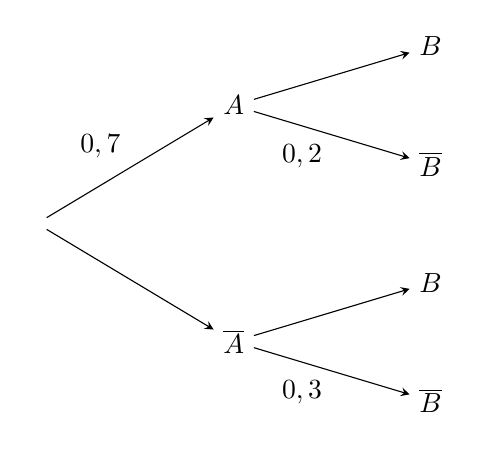
\begin{tikzpicture}[x=2.5cm, y=1.5cm]
        \node (R) at (0,0) {};
        \node (A) at (1,1) {$A$};
        \node (nA) at (1,-1) {$\overline{A}$};
        \node (B1) at (2,1.5) {$B$};
        \node (nB1) at (2,0.5) {$\overline{B}$};
        \node (B2) at (2,-0.5) {$B$};
        \node (nB2) at (2,-1.5) {$\overline{B}$};
        \draw[->,>=stealth] (R) -- (A) node[midway, above left] {$0,7$};
        \draw[->,>=stealth] (R) -- (nA) node[midway, below left] {};
        \draw[->,>=stealth] (A) -- (B1) node[midway, above left] {};
        \draw[->,>=stealth] (A) -- (nB1) node[midway, below left] {$0,2$};
        \draw[->,>=stealth] (nA) -- (B2) node[midway, above left] {};
        \draw[->,>=stealth] (nA) -- (nB2) node[midway, below left] {$0,3$};
    \end{tikzpicture}
}
   \loigiai{
       Từ sơ đồ, ta có $P(A) = 0,7 \Rightarrow P(\overline{A}) = 0,3$.\\
       $P(\overline{B}|A) = 0,2 \Rightarrow P(B|A) = 0,8$.\\
       $P(\overline{B}|\overline{A}) = 0,3 \Rightarrow P(B|\overline{A}) = 0,7$.\\
       a) $P(B|A) = 0,8$. (Đúng)\\
       b) $P(AB) = P(A) \cdot P(B|A) = 0,7 \cdot 0,8 = 0,56$. (Đúng)\\
       c) $P(\overline{A} \cap \overline{B}) = P(\overline{A}) \cdot P(\overline{B}|\overline{A}) = 0,3 \cdot 0,3 = 0,09$. Mệnh đề cho $0,21$ là sai.\\
       d) $P(B) = P(AB) + P(\overline{A} \cap B) = 0,56 + 0,3 \cdot 0,7 = 0,77$. Mệnh đề cho $0,42$ là sai.
   }
%\dotlineEX{3}
\end{ex}
\begin{ex}%[146776] [MĐ2]
    Một người có 5 con gà mái, 2 con gà trống nhốt chung trong một cái lồng. Một người đến mua, người bán gà bắt ngẫu nhiên 1 con. Người mua chấp nhận mua con gà đó. Xét tính đúng sai của các mệnh đề sau:
    \choiceTF
    {\True Xác suất để người đó mua được con gà mái là $\dfrac{5}{7}$}
    { Xác suất để người đó mua được con gà trống là $\dfrac{2}{5}$}
    {\True Một người thứ hai lại đến mua gà, người bán gà lại bắt ngẫu nhiên ra 1 con, xác suất để người thứ hai mua được con gà trống khi người thứ nhất mua được con gà mái là $\dfrac{1}{3}$}
    {Trong trường hợp người bán gà quên mất rằng con gà bán cho người thứ nhất là gà trống hay gà mái. Xác suất để người thứ hai mua được gà trống bằng $\dfrac{3}{7}$}
    \loigiai{
        Tổng số gà trong lồng là $7$ con.
        \begin{itemize}
            \item a) Xác suất bắt được gà mái lần đầu là $\dfrac{5}{7}$. (Đúng)
            \item b) Xác suất bắt được gà trống lần đầu là $\dfrac{2}{7}$. Mệnh đề cho $\dfrac{2}{5}$ là (Sai).
            \item c) Nếu người thứ nhất mua gà mái, lồng còn 4 mái, 2 trống (tổng 6 con). Xác suất người thứ hai mua được gà trống là $\dfrac{2}{6} = \dfrac{1}{3}$. (Đúng)
            \item d) Xác suất người thứ hai mua được gà trống (khi không biết người thứ nhất mua gì) tính theo công thức xác suất toàn phần:
            $$P = \dfrac{5}{7} \cdot \dfrac{2}{6} + \dfrac{2}{7} \cdot \dfrac{1}{6} = \dfrac{10}{42} + \dfrac{2}{42} = \dfrac{12}{42} = \dfrac{2}{7}.$$
            Mệnh đề cho $\dfrac{3}{7}$ là (Sai).
        \end{itemize}
    }
    %\dotlineEX{2}
\end{ex}
\begin{ex}%[144831] [MĐ3]
    Một nhà máy có hai máy I và II. Máy I sản xuất $40\%$ số lượng sản phẩm và Máy II sản xuất $60\%$ số lượng sản phẩm. Có $4\%$ mặt hàng do Máy I sản xuất bị lỗi và $5\%$ sản phẩm do Máy II sản xuất bị lỗi. Một vật phẩm được rút ngẫu nhiên. Xét tính đúng sai của các mệnh đề sau:
    \choiceTF
    {\True Nếu vật phẩm được sản xuất bởi máy I thì xác suất sản phẩm đó bị lỗi là $0,04$}
    { Xác suất để vật lấy ra được tạo bởi máy II và không bị lỗi là $0,384$}
    { Xác suất để vật lấy ra không bị lỗi là $0,046$}
    {\True Nếu vật được rút ra bị lỗi, xác suất để vật đó được tạo ra bởi Máy II bằng $\dfrac{15}{23}$}
    \loigiai{
        Gọi $M_1, M_2$ là biến cố sản phẩm do máy 1, máy 2 sản xuất $\Rightarrow P(M_1) = 0,4; P(M_2) = 0,6$.\\
        Gọi $L$ là biến cố "Sản phẩm bị lỗi". Ta có $P(L|M_1) = 0,04$ và $P(L|M_2) = 0,05$.\\
        a) Theo đúng giả thiết, xác suất này là $P(L|M_1) = 0,04$. (Đúng)\\
        b) Xác suất vật tạo bởi máy II và không bị lỗi là $P(M_2 \cap \overline{L}) = P(M_2) \cdot P(\overline{L}|M_2) = 0,6 \cdot (1 - 0,05) = 0,6 \cdot 0,95 = 0,57$. (Sai)\\
        c) Xác suất vật lấy ra bị lỗi là $P(L) = 0,4 \cdot 0,04 + 0,6 \cdot 0,05 = 0,016 + 0,030 = 0,046$. Vậy xác suất không bị lỗi là $1 - 0,046 = 0,954$. (Sai)\\
        d) Xác suất vật lỗi do máy II tạo ra: $P(M_2|L) = \dfrac{P(M_2 \cap L)}{P(L)} = \dfrac{0,030}{0,046} = \dfrac{30}{46} = \dfrac{15}{23}$. (Đúng)
    }
\end{ex}
\begin{ex}%[145264] [MĐ3]
    Một bộ lọc được sử dụng để chặn thư rác trong các tài khoản thư điện tử. Tuy nhiên, vì bộ lọc không tuyệt đối hoàn hảo nên một thư rác bị chặn với xác suất $0,95$ và một thư đúng (không phải là thư rác) bị chặn với xác suất $0,01$. Thống kê cho thấy tỉ lệ thư rác là $3\%$. Các mệnh đề sau đúng hay sai.
    \choiceTF
    {\True Xác suất để thư đó bị chặn là $3,82\%$}
    { Chọn ngẫu nhiên một thư bị chặn. Xác suất để đó là thư rác xấp xỉ $96,7\%$}
    {\True Chọn ngẫu nhiên một thư không bị chặn. Xác suất để đó là thư đúng xấp xỉ $99,84\%$}
    { Trong số các thư không bị chặn, có xấp xỉ $1,56\%$ là thư rác}
    \loigiai{
        Gọi $R$ là biến cố "Thư rác", $P(R) = 0,03 \Rightarrow P(\text{Thư đúng}) = P(\overline{R}) = 0,97$.\\
        Gọi $C$ là biến cố "Thư bị chặn". Ta có $P(C|R) = 0,95$ và $P(C|\overline{R}) = 0,01$.\\
        a) Xác suất thư bị chặn $P(C) = 0,03 \cdot 0,95 + 0,97 \cdot 0,01 = 0,0285 + 0,0097 = 0,0382 = 3,82\%$. (Đúng)\\
        b) Xác suất là thư rác biết đã bị chặn: $P(R|C) = \dfrac{0,0285}{0,0382} \approx 0,746 = 74,6\%$. (Sai)\\
        c) Xác suất là thư đúng khi không bị chặn: $P(\overline{R}|\overline{C}) = \dfrac{P(\overline{R} \cap \overline{C})}{P(\overline{C})} = \dfrac{0,97 \cdot (1 - 0,01)}{1 - 0,0382} = \dfrac{0,97 \cdot 0,99}{0,9618} = \dfrac{0,9603}{0,9618} \approx 0,9984 = 99,84\%$. (Đúng)\\
        d) Xác suất là thư rác trong số thư không bị chặn: $P(R|\overline{C}) = 1 - P(\overline{R}|\overline{C}) = 1 - 0,9984 = 0,0016 = 0,16\%$. (Sai)
    }
\end{ex}
\begin{ex}%[144879] [MĐ3]
    Có 6 khẩu súng cũ và 4 khẩu súng mới, trong đó xác suất trúng khi bắn bằng súng cũ là $0,8$, còn súng mới là $0,95$. Một người lấy ngẫu nhiên một khẩu súng và bắn một mục tiêu. Các mệnh đề sau đúng hay sai.
    \choiceTF
    {\True Xác suất để người đó bắn khẩu súng cũ là $0,6$}
    { Xác suất để người đó bắn khẩu súng mới và trúng mục tiêu là $0,57$}
    {\True Xác suất để người đó bắn trúng mục tiêu là $0,86$}
    { Giả sử người đó bắn trúng mục tiêu thì xác suất người đó dùng súng mới là cao hơn}
    \loigiai{
        Tổng có 10 khẩu súng. Xác suất chọn súng cũ là $P(C) = 0,6$, súng mới là $P(M) = 0,4$.\\
        Gọi $T$ là biến cố "Bắn trúng mục tiêu". $P(T|C) = 0,8$ và $P(T|M) = 0,95$.\\
        a) $P(C) = 0,6$. (Đúng)\\
        b) $P(M \cap T) = P(M)P(T|M) = 0,4 \cdot 0,95 = 0,38$. (Sai)\\
        c) $P(T) = 0,6 \cdot 0,8 + 0,4 \cdot 0,95 = 0,48 + 0,38 = 0,86$. (Đúng)\\
        d) Nếu bắn trúng, xác suất dùng súng mới là $P(M|T) = \dfrac{0,38}{0,86} \approx 0,44$. Xác suất dùng súng cũ là $P(C|T) = \dfrac{0,48}{0,86} \approx 0,56$. Khả năng dùng súng cũ cao hơn. (Sai)
    }
\end{ex}
\begin{ex}%[144885] [MĐ3]
    Trong một trạm cấp cứu bỏng: $80\%$ bệnh nhân bỏng do nóng, $20\%$ bỏng do hóa chất. Loại bỏng do nóng có $30\%$ bị biến chứng, loại bỏng do hóa chất có $50\%$ bị biến chứng. Các mệnh đề sau đúng hay sai.
    \choiceTF
    {\True Loại bỏng do nóng có $70\%$ không bị biến chứng}
    { Chọn ngẫu nhiên một bệnh án. Xác suất để gặp bệnh án của bệnh nhân bị bỏng nóng và không bị biến chứng là $0,4$}
    {\True Chọn ngẫu nhiên một bệnh án. Xác suất để gặp một bệnh án của bệnh nhân bị biến chứng là $0,34$}
    { Rút ngẫu nhiên được một bệnh án của một bệnh nhân bị biến chứng. Xác suất để bệnh án đó là của bệnh nhân bị biến chứng do hoá chất gây ra là $\dfrac{12}{17}$}
   \loigiai{
       Gọi $N$ là "Bỏng do nóng", $H$ là "Bỏng do hóa chất" $\Rightarrow P(N) = 0,8; P(H) = 0,2$.\\
       Gọi $B$ là biến cố "Bị biến chứng". $P(B|N) = 0,3$ và $P(B|H) = 0,5$.\\
       a) Tỷ lệ bỏng do nóng không biến chứng là $1 - P(B|N) = 1 - 0,3 = 0,7 = 70\%$. (Đúng)\\
       b) Bỏng nóng và không biến chứng: $P(N \cap \overline{B}) = P(N)P(\overline{B}|N) = 0,8 \cdot 0,7 = 0,56$. (Sai)\\
       c) Xác suất gặp bệnh án bị biến chứng: $P(B) = 0,8 \cdot 0,3 + 0,2 \cdot 0,5 = 0,24 + 0,10 = 0,34$. (Đúng)\\
       d) Xác suất do hóa chất khi biết bị biến chứng: $P(H|B) = \dfrac{P(H \cap B)}{P(B)} = \dfrac{0,10}{0,34} = \dfrac{10}{34} = \dfrac{5}{17}$. (Sai)
   }
\end{ex}
\begin{ex}%[144894] [MĐ3]
    Một công ty xây dựng có 2 kỹ sư điều hành. Kỹ sư-1 thực hiện $60\%$ công việc của công ty. Kỹ sư-2 thực hiện $40\%$ công việc của công ty. Kinh nghiệm trước đây cho thấy xác suất xảy ra sai sót khi kỹ sư 1 thực hiện công việc là $0,03$, trong khi xác suất xảy ra sai sót trong công việc của kỹ sư 2 là $0,04$. Các mệnh đề sau đúng hay sai.
    \choiceTF
    { Xác suất để một công việc do kĩ sư 1 thực hiện và không xảy ra lỗi là $0,388$}
    {\True Xác suất để xảy ra một lỗi trong công việc là $0,034$}
    { Giả sử xảy ra một lỗi trong công việc, xác suất để lỗi đó do kỹ sư 1 thực hiện là $\dfrac{8}{17}$}
    {\True Giả sử xảy ra một lỗi trong công việc, thì xác suất xảy ra lỗi của kỹ sư 1 lớn hơn khả năng xảy ra lỗi của kỹ sư 2}
    \loigiai{
        Gọi $K_1, K_2$ là biến cố công việc do kỹ sư 1, kỹ sư 2 thực hiện. $P(K_1) = 0,6; P(K_2) = 0,4$.\\
        Gọi $L$ là biến cố "Xảy ra lỗi". $P(L|K_1) = 0,03$ và $P(L|K_2) = 0,04$.\\
        a) Công việc do kỹ sư 1 và không lỗi: $P(K_1 \cap \overline{L}) = 0,6 \cdot (1 - 0,03) = 0,6 \cdot 0,97 = 0,582$. (Sai)\\
        b) Xác suất xảy ra lỗi: $P(L) = 0,6 \cdot 0,03 + 0,4 \cdot 0,04 = 0,018 + 0,016 = 0,034$. (Đúng)\\
        c) Lỗi do kỹ sư 1 thực hiện: $P(K_1|L) = \dfrac{P(K_1 \cap L)}{P(L)} = \dfrac{0,018}{0,034} = \dfrac{18}{34} = \dfrac{9}{17}$. (Sai)\\
        d) Lỗi do kỹ sư 2 thực hiện là $P(K_2|L) = \dfrac{0,016}{0,034} = \dfrac{8}{17}$. Ta thấy $\dfrac{9}{17} > \dfrac{8}{17}$. (Đúng)
    }
    %\dotlineEX{2}
\end{ex}
\begin{ex}%[145230] [MĐ3]
    Một công ty đấu thầu 2 dự án. Khả năng thắng thầu của các dự án 1 và 2 lần lượt là $0,4$ và $0,5$. Khả năng thắng thầu cả 2 dự án là $0,3$. Gọi A, B lần lượt là biến cố thắng thầu dự án 1 và dự án 2. Các mệnh đề sau đúng hay sai.
    \choiceTF
    { A và B là hai biến cố độc lập}
    {\True Xác suất để công ty thắng thầu đúng một dự án là $0,3$}
    {\True Biết công ty thắng thầu dự án 1, xác suất công ty thắng thầu dự án 2 là $0,75$}
    { Biết công ty không thắng thầu dự án 1, xác suất công ty thắng thầu dự án 2 là $0,5$}
    \loigiai{
        Ta có $P(A) = 0,4; P(B) = 0,5$ và $P(A \cap B) = 0,3$.\\
        a) Nếu A, B độc lập thì $P(A)P(B) = P(A \cap B) \Leftrightarrow 0,4 \cdot 0,5 = 0,2 \ne 0,3$. Do đó A và B không độc lập. (Sai)\\
        b) Thắng đúng 1 dự án: $P(A \cap \overline{B}) + P(\overline{A} \cap B) = [P(A) - P(A \cap B)] + [P(B) - P(A \cap B)] = (0,4 - 0,3) + (0,5 - 0,3) = 0,1 + 0,2 = 0,3$. (Đúng)\\
        c) Xác suất thắng DA 2 khi biết thắng DA 1: $P(B|A) = \dfrac{P(A \cap B)}{P(A)} = \dfrac{0,3}{0,4} = 0,75$. (Đúng)\\
        d) Xác suất thắng DA 2 khi biết không thắng DA 1: $P(B|\overline{A}) = \dfrac{P(B \cap \overline{A})}{P(\overline{A})} = \dfrac{0,2}{1 - 0,4} = \dfrac{0,2}{0,6} = \dfrac{1}{3} \approx 0,33$. (Sai)
    }
    %\dotlineEX{2}
\end{ex}
\begin{ex}%[145231] [MĐ3]
    Một học sinh làm 2 bài tập kế tiếp. Xác suất làm đúng bài thứ nhất là $0,7$. Nếu làm đúng bài thứ nhất thì khả năng làm đúng bài thứ 2 là $0,8$, nhưng nếu làm sai bài thứ 1 thì khả năng làm đúng bài thứ 2 là $0,2$. Các mệnh đề sau đúng hay sai.
    \choiceTF
    {\True Xác suất làm sai bài thứ nhất là $0,3$}
    {\True Xác suất làm đúng ít nhất 1 bài là $0,76$}
    { Xác suất làm đúng bài 1 biết rằng làm đúng bài 2 là $0,8$}
    {\True Xác suất làm đúng cả 2 bài, biết rằng làm đúng ít nhất một bài là $\dfrac{14}{19}$}
    \loigiai{
        Gọi $D_1, D_2$ là biến cố làm đúng bài 1, bài 2. $P(D_1) = 0,7 \Rightarrow P(\overline{D_1}) = 0,3$.\\
        Ta có $P(D_2|D_1) = 0,8$ và $P(D_2|\overline{D_1}) = 0,2$.\\
        a) Xác suất sai bài 1 là $1 - 0,7 = 0,3$. (Đúng)\\
        b) Làm đúng ít nhất 1 bài bằng phần bù của làm sai cả 2 bài: $1 - P(\overline{D_1} \cap \overline{D_2}) = 1 - P(\overline{D_1})P(\overline{D_2}|\overline{D_1}) = 1 - 0,3 \cdot (1 - 0,2) = 1 - 0,24 = 0,76$. (Đúng)\\
        c) $P(D_2) = 0,7 \cdot 0,8 + 0,3 \cdot 0,2 = 0,56 + 0,06 = 0,62$.\\
        $P(D_1|D_2) = \dfrac{P(D_1 \cap D_2)}{P(D_2)} = \dfrac{0,56}{0,62} = \dfrac{28}{31}$. Mệnh đề cho 0,8 là (Sai)\\
        d) Đúng 2 bài biết đúng ít nhất 1 bài: $\dfrac{P(D_1 \cap D_2)}{P(\text{Ít nhất 1 bài})} = \dfrac{0,56}{0,76} = \dfrac{56}{76} = \dfrac{14}{19}$. (Đúng)
    }
    %\dotlineEX{3}
\end{ex}
\begin{ex}[KSCL12-Sở Quảng Ninh-2026]
    Một trung tâm ngoại ngữ tổ chức một kỳ thi đánh giá năng lực cho các học viên. Trung tâm thống kê được rằng:
    \begin{itemize}
        \item $55\%$ thí sinh là nữ;
        \item trong số các thí sinh nữ có $80\%$ thí sinh vượt qua bài kiểm tra;
        \item trong số các thí sinh nam có $25\%$ thí sinh không vượt qua bài kiểm tra.
    \end{itemize}
    Chọn ngẫu nhiên một thí sinh.
    \choiceTF
    {\True Xác suất để thí sinh được chọn là nam bằng $0,45$}
    {\True Xác suất để thí sinh được chọn vượt qua bài kiểm tra, biết rằng thí sinh đó là nam, bằng $0,75$}
    {Xác suất để thí sinh được chọn vượt qua bài kiểm tra bằng $77,25\%$}
    { Xác suất để thí sinh được chọn là nữ, biết rằng thí sinh đó không vượt qua bài kiểm tra, nhỏ hơn $0,45$}
    \loigiai{
        Gọi $A$ là biến cố ``Thí sinh được chọn là nam'' và $B$ là biến cố ``Thí sinh được chọn vượt qua bài kiểm tra''.\\
        Suy ra $\overline{A}$ là biến cố ``Thí sinh được chọn là nữ'' và $\overline{B}$ là biến cố ``Thí sinh không vượt qua bài kiểm tra''.
        \begin{itemize}
            \item Từ (1), ta có $P(\overline{A}) = 0,55 \Rightarrow P(A) = 1 - 0,55 = 0,45$. \textbf{Vậy mệnh đề a đúng}.
            \item Từ (2), ta có $P(B|\overline{A}) = 0,8 \Rightarrow P(\overline{B}|\overline{A}) = 1 - 0,8 = 0,2$.
            \item Từ (3), ta có $P(\overline{B}|A) = 0,25 \Rightarrow P(B|A) = 1 - 0,25 = 0,75$. \textbf{Vậy mệnh đề b đúng}.
        \end{itemize}
        Xác suất để thí sinh được chọn vượt qua bài kiểm tra là:
        $$P(B) = P(A) \cdot P(B|A) + P(\overline{A}) \cdot P(B|\overline{A}) = 0,45 \cdot 0,75 + 0,55 \cdot 0,8 = 0,7775 = 77,75\%.$$
        \textbf{Vậy mệnh đề c sai}.\\
        Xác suất thí sinh là nữ, biết rằng thí sinh đó không vượt qua bài kiểm tra là:
        $$P(\overline{A}|\overline{B}) = \dfrac{P(\overline{A}) \cdot P(\overline{B}|\overline{A})}{P(\overline{B})} = \dfrac{0,55 \cdot 0,2}{1 - 0,7775} = \dfrac{0,11}{0,2225} \approx 0,494 > 0,45.$$
        \textbf{Vậy mệnh đề d sai}.
    }
    %\dotlineEX{2}
\end{ex}
\begin{ex}%[360662] [MĐ2]
    Một công ty dược phẩm giới thiệu một dụng cụ kiểm tra sớm bệnh sốt xuất huyết. Về kiểm định chất lượng sản phẩm, họ cho biết như sau: Số người được thử là $9000$, trong số đó có $1500$ người đã bị nhiễm bệnh sốt xuất huyết và có $7500$ người không bị nhiễm bệnh sốt xuất huyết. Khi thử bằng dụng cụ của công ty, trong $1500$ người đã bị nhiễm bệnh sốt xuất huyết, có 76\% số người đó cho kết quả dương tính, còn lại cho kết quả âm tính. Mặt khác, trong $7500$ người không bị nhiễm bệnh sốt xuất huyết, có 7\% số người đó cho kết quả dương tính, còn lại cho kết quả âm tính khi kiểm tra. Chọn ngẫu nhiên một người trong số những người thử nghiệm. Tính xác suất để người được chọn ra bị nhiễm bệnh sốt xuất huyết, biết rằng người đó có kết quả thử nghiệm âm tính (làm tròn kết quả đến hàng phần trăm).
    \shortans{$0,05$}
    \loigiai{
        Gọi $B$ là biến cố người đó nhiễm bệnh $\Rightarrow P(B) = \dfrac{1500}{9000} = \dfrac{1}{6}$; $P(\overline{B}) = \dfrac{7500}{9000} = \dfrac{5}{6}$.\\
        Gọi $A$ là biến cố kết quả thử âm tính. Ta có $P(A|B) = 1 - 0,76 = 0,24$ và $P(A|\overline{B}) = 1 - 0,07 = 0,93$.\\
        Xác suất âm tính: $P(A) = P(B)P(A|B) + P(\overline{B})P(A|\overline{B}) = \dfrac{1}{6} \cdot 0,24 + \dfrac{5}{6} \cdot 0,93 = 0,04 + 0,775 = 0,815$.\\
        Xác suất bị nhiễm bệnh khi âm tính: $P(B|A) = \dfrac{P(B \cap A)}{P(A)} = \dfrac{0,04}{0,815} \approx 0,04907 \approx 0,05$.
    }
    %\dotlineEX{1}
\end{ex}
\begin{ex}%[135784] [MĐ2]
    Trên giá sách có 10 quyển sách Khoa học và 15 quyển sách Nghệ thuật. Có 9 quyển sách viết bằng tiếng Anh, trong đó 3 quyển sách Khoa học và 6 quyển sách Nghệ thuật, các quyển sách còn lại viết bằng tiếng Việt. Lấy ngẫu nhiên một quyển sách. Tính xác suất để quyển sách được lấy ra là sách viết bằng tiếng Việt, biết rằng quyển sách đó là sách Khoa học.
    \shortans{$0,7$}
    \loigiai{
        Có tổng cộng 10 quyển sách Khoa học.\\
        Số sách Khoa học viết bằng tiếng Anh là 3 quyển. Do đó, số sách Khoa học viết bằng tiếng Việt là $10 - 3 = 7$ quyển.\\
        Xác suất lấy được sách tiếng Việt biết đó là sách Khoa học là $P = \dfrac{7}{10} = 0,7$.
    }
    %\dotlineEX{1}
\end{ex}
\begin{ex}%[135859] [MĐ2]
    Trong một hộp kín có 7 chiếc bút bi xanh và 5 chiếc bút bi đen, các chiếc bút có cùng kích thước và khối lượng. Bạn Sơn lấy ngẫu nhiên một chiếc bút bi từ trong hộp, không trả lại. Sau đó bạn Tùng lấy ngẫu nhiên một trong 11 chiếc bút còn lại. Tính xác suất để hai chiếc bút lấy ra có cùng màu. Viết kết quả làm tròn đến hàng phần trăm.
    \shortans{$0,47$}
    \loigiai{
        Hai chiếc bút cùng màu khi cả hai đều xanh hoặc cả hai đều đen.\\
        - Xác suất cả 2 bút màu xanh: $\dfrac{7}{12} \cdot \dfrac{6}{11} = \dfrac{42}{132}$.\\
        - Xác suất cả 2 bút màu đen: $\dfrac{5}{12} \cdot \dfrac{4}{11} = \dfrac{20}{132}$.\\
        Xác suất lấy 2 bút cùng màu là $P = \dfrac{42 + 20}{132} = \dfrac{62}{132} = \dfrac{31}{66} \approx 0,4696 \approx 0,47$.
    }
\end{ex}
\begin{ex}%[378716] [MĐ2]
    Trong một túi có một số chiếc kẹo cùng loại, chỉ khác màu, trong đó có 6 cái kẹo màu cam, còn lại là kẹo màu vàng. Hà lấy ngẫu nhiên một cái kẹo từ trong túi, không trả lại. Sau đó Hà lại lấy ngẫu nhiên thêm một cái kẹo khác từ trong túi. Biết rằng xác suất Hà lấy được cả hai cái kẹo màu cam là $\dfrac{1}{3}$. Hỏi ban đầu trong túi có bao nhiêu cái kẹo?
    \shortans{$10$}
    \loigiai{
        Gọi tổng số kẹo ban đầu là $N$ ($N \ge 2, N \in \mathbb{N}^*$).\\
        Xác suất lấy được 2 cái kẹo màu cam liên tiếp (không hoàn lại) là: $\dfrac{6}{N} \cdot \dfrac{5}{N-1}$.\\
        Theo bài ra ta có: $\dfrac{30}{N(N-1)} = \dfrac{1}{3} \Leftrightarrow N(N-1) = 90 \Leftrightarrow N^2 - N - 90 = 0$.\\
        Giải phương trình ta được $N = 10$ (nhận) hoặc $N = -9$ (loại).\\
        Vậy ban đầu trong túi có 10 cái kẹo.
    }
    %\dotlineEX{1}
\end{ex}
\begin{ex}%[143811] [MĐ2]
    Có 2 xạ thủ loại I và 8 xạ thủ loại II, xác suất bắn trúng đích của các loại xạ thủ loại I là 0,9 và loại II là 0,7. Chọn ngẫu nhiên ra một xạ thủ và xạ thủ đó bắn một viên đạn. Tìm xác suất để viên đạn đó trúng đích.
    \shortans{$0,74$}
    \loigiai{
        Tổng số xạ thủ là 10. Xác suất chọn được xạ thủ loại I là $P(\text{I}) = \dfrac{2}{10} = 0,2$. Xác suất chọn được xạ thủ loại II là $P(\text{II}) = \dfrac{8}{10} = 0,8$.\\
        Xác suất viên đạn trúng đích là:
        $$P(\text{Trúng}) = 0,2 \cdot 0,9 + 0,8 \cdot 0,7 = 0,18 + 0,56 = 0,74.$$
    }
\end{ex}
\begin{ex}%[143812] [MĐ2]
    Theo thống kê xác suất để hai ngày liên tiếp có mưa ở một thành phố vào mùa hè là 0,5; còn không mưa là 0,3. Biết các sự kiện có một ngày mưa, một ngày không mưa là đồng khả năng. Tính xác suất để ngày thứ hai có mưa, biết ngày đầu không mưa.
    \shortans{$0,25$}
    \loigiai{
        Gọi (Mưa, Mưa) là RR, (Không, Không) là NN, (Mưa, Không) là RN, (Không, Mưa) là NR.\\
        Theo giả thiết: $P(RR) = 0,5$; $P(NN) = 0,3$; $P(RN) = P(NR)$.\\
        Vì tổng xác suất bằng 1 nên $0,5 + 0,3 + 2P(NR) = 1 \Rightarrow 2P(NR) = 0,2 \Rightarrow P(NR) = 0,1$.\\
        Xác suất ngày đầu không mưa là: $P(\text{Ngày 1 N}) = P(NN) + P(NR) = 0,3 + 0,1 = 0,4$.\\
        Xác suất ngày thứ hai mưa, biết ngày đầu không mưa là:
        $$P(\text{Ngày 2 R} \mid \text{Ngày 1 N}) = \dfrac{P(NR)}{P(\text{Ngày 1 N})} = \dfrac{0,1}{0,4} = 0,25.$$
    }
    %\dotlineEX{1}
\end{ex}
\begin{ex}%[378735] [MĐ2]
    Chuồng I có 5 con gà mái, 2 con gà trống. Chuồng II có 3 con gà mái, 5 con gà trống. Bác Mai bắt một con gà trong số đó theo cách sau: "Bác tung một con xúc xắc cân đối, đồng chất. Nếu số chấm chia hết cho 3 thì bác chọn chuồng I. Nếu số chấm không chia hết cho 3 thì bác chọn chuồng II. Sau đó, từ chuồng đã chọn bác bắt ngẫu nhiên một con gà". Tính xác suất để bác Mai bắt được con gà mái. Viết kết quả làm tròn đến hàng phần trăm.
    \shortans{$0,49$}
    \loigiai{
        Xác suất xúc xắc ra số chấm chia hết cho 3 (mặt 3, 6) là $P(\text{C I}) = \dfrac{2}{6} = \dfrac{1}{3}$.\\
        Xác suất ra số chấm không chia hết cho 3 (mặt 1, 2, 4, 5) là $P(\text{C II}) = \dfrac{4}{6} = \dfrac{2}{3}$.\\
        Xác suất bắt được gà mái:
        $$P(\text{Mái}) = P(\text{C I})P(\text{Mái} \mid \text{C I}) + P(\text{C II})P(\text{Mái} \mid \text{C II}) = \dfrac{1}{3} \cdot \dfrac{5}{7} + \dfrac{2}{3} \cdot \dfrac{3}{8} = \dfrac{5}{21} + \dfrac{1}{4} = \dfrac{41}{84} \approx 0,488.$$
        Làm tròn đến hàng phần trăm ta được $0,49$.
    }
    %\dotlineEX{1}
\end{ex}
\begin{ex}%[143814] [MĐ2]
    Có 2 hộp áo; hộp một có 10 áo trong đó có 1 phế phẩm; hộp hai có 8 áo trong đó có 2 phế phẩm. Lấy ngẫu nhiên 1 áo từ hộp một bỏ sang hộp hai; sau đó từ hộp này chọn ngẫu nhiên ra 2 áo. Gọi $p$ là xác suất để cả 2 áo này đều là phế phẩm. Tính $\dfrac{1}{p}$.
    \shortans{$30$}
    \loigiai{
        Xác suất chuyển 1 áo phế phẩm từ hộp một sang hộp hai là $\dfrac{1}{10}$. Khi đó hộp hai có 3 phế phẩm, 6 áo tốt (tổng 9). Xác suất lấy ra 2 phế phẩm là $\dfrac{C_3^2}{C_9^2} = \dfrac{3}{36}$.\\
        Xác suất chuyển 1 áo tốt là $\dfrac{9}{10}$. Khi đó hộp hai có 2 phế phẩm, 7 áo tốt. Xác suất lấy ra 2 phế phẩm là $\dfrac{C_2^2}{C_9^2} = \dfrac{1}{36}$.\\
        Xác suất $p$:
        $$p = \dfrac{1}{10} \cdot \dfrac{3}{36} + \dfrac{9}{10} \cdot \dfrac{1}{36} = \dfrac{3+9}{360} = \dfrac{12}{360} = \dfrac{1}{30}.$$
        Vậy $\dfrac{1}{p} = 30$.
    }
\end{ex}
\begin{ex}%[378722] [MĐ3]
    Trong quân sự, một máy bay chiến đấu của đối phương có thể xuất hiện ở vị trí X với xác suất 0,55. Nếu máy bay đó không xuất hiện ở vị trí X thì nó xuất hiện ở vị trí Y. Để phòng thủ, các bệ phóng tên lửa được bố trí tại các vị trí X và Y. Khi máy bay đối phương xuất hiện ở vị trí X hoặc Y thì tên lửa sẽ được phóng để hạ máy bay đó.
    Xét phương án tác chiến sau: Nếu máy bay xuất hiện tại X thì bắn 2 quả tên lửa và nếu máy bay xuất hiện tại Y thì bắn một quả tên lửa. Biết rằng, xác suất bắn trúng máy bay của mỗi quả tên lửa là 0,8 và các bệ phóng tên lửa hoạt động độc lập. Máy bay bị bắn hạ nếu nó trúng ít nhất 1 quả tên lửa. Tính xác suất bắn hạ máy bay đối phương trong phương án tác chiến nêu trên. Viết kết quả làm tròn đến hàng phần trăm.
    \shortans{$0,89$}
    \loigiai{
        Xác suất máy bay ở X là $0,55$. Ở Y là $1 - 0,55 = 0,45$.\\
        Nếu ở X, bắn 2 tên lửa. Xác suất trượt cả 2 là $(1 - 0,8)^2 = 0,04$. Xác suất hạ được là $1 - 0,04 = 0,96$.\\
        Nếu ở Y, bắn 1 tên lửa. Xác suất hạ được là $0,8$.\\
        Xác suất hạ được máy bay:
        $$P = 0,55 \cdot 0,96 + 0,45 \cdot 0,8 = 0,528 + 0,36 = 0,888.$$
        Làm tròn đến hàng phần trăm ta được $0,89$.
    }
    %\dotlineEX{1}
\end{ex}
\begin{ex}%[143815] [MĐ3]
    Một chiếc máy bay có thể xuất hiện ở vị trí A với xác suất $\dfrac{2}{3}$ và ở vị trí B với xác suất $\dfrac{1}{3}$. Người ta đặt 3 khẩu súng ở vị trí A và 1 khẩu súng ở vị trí B. Biết rằng xác suất bắn trúng máy bay của mỗi khẩu pháo là 0,7 và các khẩu pháo hoạt động độc lập với nhau, tính xác suất máy bay rơi, biết rằng máy bay sẽ rơi nếu bị bắn trúng. Viết kết quả làm tròn đến hàng phần trăm.
    \shortans{$0,88$}
    \loigiai{
        Nếu máy bay ở A (xác suất $\dfrac{2}{3}$): Bị bắn bởi 3 khẩu. Xác suất trượt cả 3 là $(1 - 0,7)^3 = 0,3^3 = 0,027$. Xác suất rơi là $1 - 0,027 = 0,973$.\\
        Nếu máy bay ở B (xác suất $\dfrac{1}{3}$): Bị bắn bởi 1 khẩu. Xác suất rơi là $0,7$.\\
        Xác suất máy bay rơi:
        $$P = \dfrac{2}{3} \cdot 0,973 + \dfrac{1}{3} \cdot 0,7 = \dfrac{1,946 + 0,7}{3} = \dfrac{2,646}{3} = 0,882.$$
        Làm tròn đến hàng phần trăm ta được $0,88$.
    }
    %\dotlineEX{1}
\end{ex}
\begin{ex}%[143816] [MĐ3]
    Một cặp trẻ sinh đôi có thể do cùng một trứng hay do hai trứng khác nhau sinh ra. Các cặp sinh đôi cùng trứng luôn có cùng giới tính. Cặp sinh đôi khác trứng thì giới tính của mỗi đứa độc lập với nhau và có xác suất 0,5 là con trai. Thống kê cho thấy 34\% cặp sinh đôi đều là trai, 30\% cặp sinh đôi đều là gái và 36\% cặp sinh đôi có giới tính khác nhau. Tìm tỷ lệ cặp sinh đôi cùng trứng.
    \shortans{$28$}
    \loigiai{
        Gọi $p$ là tỷ lệ cặp sinh đôi cùng trứng, khi đó tỷ lệ cặp sinh đôi khác trứng là $1 - p$.\\
        Cặp sinh đôi có giới tính khác nhau chỉ xảy ra ở trường hợp sinh đôi khác trứng.\\
        Xác suất sinh đôi khác trứng mà 1 trai 1 gái là $2 \cdot 0,5 \cdot 0,5 = 0,5$.\\
        Theo đề bài, xác suất sinh ra cặp có giới tính khác nhau là 36\%, do đó:
        $$(1 - p) \cdot 0,5 = 0,36 \Rightarrow 1 - p = 0,72 \Rightarrow p = 0,28 = 28\%.$$
        Vậy tỷ lệ cặp sinh đôi cùng trứng là 28\%.
    }
    %\dotlineEX{1}
\end{ex}
\begin{ex}%[143813] [MĐ3]
    Có 2 hộp đựng sản phẩm. Hộp thứ nhất có 10 sản phẩm trong đó có 9 sản phẩm tốt và 1 sản phẩm xấu. Hộp thứ hai có 20 sản phẩm trong đó có 18 sản phẩm tốt và 2 sản phẩm xấu. Từ hộp thứ nhất lấy ngẫu nhiên một sản phẩm bỏ sang hộp thứ hai. Tìm xác suất để lấy ngẫu nhiên một sản phẩm từ hộp thứ hai được sản phẩm tốt.
    \shortans{$0,9$}
    \loigiai{
        Xác suất chuyển 1 sản phẩm tốt từ hộp thứ nhất sang hộp thứ hai là $\dfrac{9}{10}$. Khi đó hộp thứ hai có 19 tốt, 2 xấu (tổng 21). Xác suất lấy được sản phẩm tốt là $\dfrac{19}{21}$.\\
        Xác suất chuyển 1 sản phẩm xấu là $\dfrac{1}{10}$. Khi đó hộp thứ hai có 18 tốt, 3 xấu (tổng 21). Xác suất lấy được sản phẩm tốt là $\dfrac{18}{21}$.\\
        Xác suất cần tìm:
        $$P = \dfrac{9}{10} \cdot \dfrac{19}{21} + \dfrac{1}{10} \cdot \dfrac{18}{21} = \dfrac{171 + 18}{210} = \dfrac{189}{210} = \dfrac{9}{10} = 0,9.$$
    }
    %\dotlineEX{2}
\end{ex}
\begin{ex}%[145259] [MĐ3]
    Có hai hộp đựng các viên bi cùng kích thước và khối lượng. Hộp thứ nhất chứa 5 viên bi đỏ và 5 viên bi xanh, hộp thứ hai chứa 6 viên bi đỏ và 4 viên bi xanh. Lấy ngẫu nhiên một viên bi từ hộp thứ nhất chuyển sang hộp thứ hai, sau đó lấy ra ngẫu nhiên một viên bi từ hộp thứ hai. Tính xác suất để viên bi được lấy ra từ hộp thứ hai là viên bi đỏ. Viết kết quả làm tròn đến hàng phần trăm.
    \shortans{$0,59$}
    \loigiai{
        Xác suất chuyển 1 viên bi đỏ từ hộp thứ nhất là $\dfrac{5}{10} = 0,5$. Hộp thứ hai sẽ có 7 đỏ, 4 xanh (tổng 11). Xác suất rút được bi đỏ là $\dfrac{7}{11}$.\\
        Xác suất chuyển 1 viên bi xanh từ hộp thứ nhất là $\dfrac{5}{10} = 0,5$. Hộp thứ hai sẽ có 6 đỏ, 5 xanh (tổng 11). Xác suất rút được bi đỏ là $\dfrac{6}{11}$.\\
        Xác suất cần tìm:
        $$P = 0,5 \cdot \dfrac{7}{11} + 0,5 \cdot \dfrac{6}{11} = \dfrac{13}{22} \approx 0,5909.$$
        Làm tròn đến hàng phần trăm ta được $0,59$.
    }
    %\dotlineEX{4}
\end{ex}
\begin{ex}%[145233] [MĐ3]
    Trong một cuộc khảo sát về việc có chơi thể thao hay không có $40\%$ nam và $60\%$ nữ tham gia. Kết quả cho thấy có $30\%$ nam và $50\%$ nữ không chơi thể thao. Chọn ngẫu nhiên một người trong số người được khảo sát. Biết người đó chơi thể thao. Tính xác suất để người được chọn là nam. Viết kết quả làm tròn đến hàng phần trăm.
    \shortans{$0,48$}
    \loigiai{
        Gọi $N$ là biến cố chọn được Nam, $P(N) = 0,4 \Rightarrow P(\text{Nữ}) = 0,6$.\\
        Gọi $C$ là biến cố "Có chơi thể thao". Ta có $P(\overline{C}|N) = 0,3 \Rightarrow P(C|N) = 0,7$.\\
        Tương tự, $P(\overline{C}|\text{Nữ}) = 0,5 \Rightarrow P(C|\text{Nữ}) = 0,5$.\\
        Xác suất chọn được người có chơi thể thao:
        $$P(C) = 0,4 \cdot 0,7 + 0,6 \cdot 0,5 = 0,28 + 0,30 = 0,58.$$
        Xác suất người đó là nam biết rằng có chơi thể thao:
        $$P(N|C) = \dfrac{P(N \cap C)}{P(C)} = \dfrac{0,28}{0,58} = \dfrac{14}{29} \approx 0,4827.$$
        Làm tròn kết quả đến hàng phần trăm ta được $0,48$.
    }
    %\dotlineEX{4}
\end{ex}

\Closesolutionfile{ans}